\section{Introduction}
\label{introduction}
In April 2008 \cite{app-engine-intro}, Google launched a platform for building
and hosting web applications on their infrastructure, called the \emph{Google App
Engine} \cite{app-engine-www}. Based on cloud computing technology, Google App
Engine uses multiple servers to run an application and store data. In addition,
Google automatically adjusts the number of servers to handle requests
simultaneously. All is offered for free by Google, provided that there are
certain quotas (e.g. bandwidth, disk space, etc.). In addition, one could
choose to sign up for a billable account, where one is billed after the quota
is exceeded.

As far as we know, the Google App Engine has not been used for scientific
purposes, similar to our project. Therefore our research question is: \emph{``To
what extent can we use the Google App Engine for scientific purposes, with
respect to Ibis?''}. Since the Google App Engine runs our applications in a
sandbox (i.e. a secure environment that provides limited access to the underlying
operating system) \cite{app-engine-sandbox}, one of the most usable parts of the
App Engine is the distributed database, called the \emph{datastore}. The
datatsore is a schemaless object datastore, with a query engine and atomic
transactions. The Python interface includes a rich data modeling API and a
SQL-like query language called GQL \cite{app-engine-datastore}.

We found that The Google App Engine datastore could well serve as an
\emph{application storage service} (also known as \emph{Advert server} -- from
now on we will use these two terms interchangeably). Its powerful query engine
and its atomic transactions makes it well suitable for storing and retrieving
Application data. For example, imagine us to have some sort of computational
workflow, where the output of each unit is the input of the next unit (see Figure
\ref{img-workflow}). Now suppose we want to store the output of the first unit,
in our example the Gaussian Blur, in order for another to find it, and continue
processing. To achieve this we will set up a central application storage service
(called the Advert server), at which we can store intermediate workflow output,
in order for other units (i.e. the Photocopy FX) to find and process it again.
This is just a basic example of what an application storage service could be used
for. Real-world examples might be more complex.

\begin{figure*}[ht] %[placement] where placement is h,t,b,p
\begin{center}
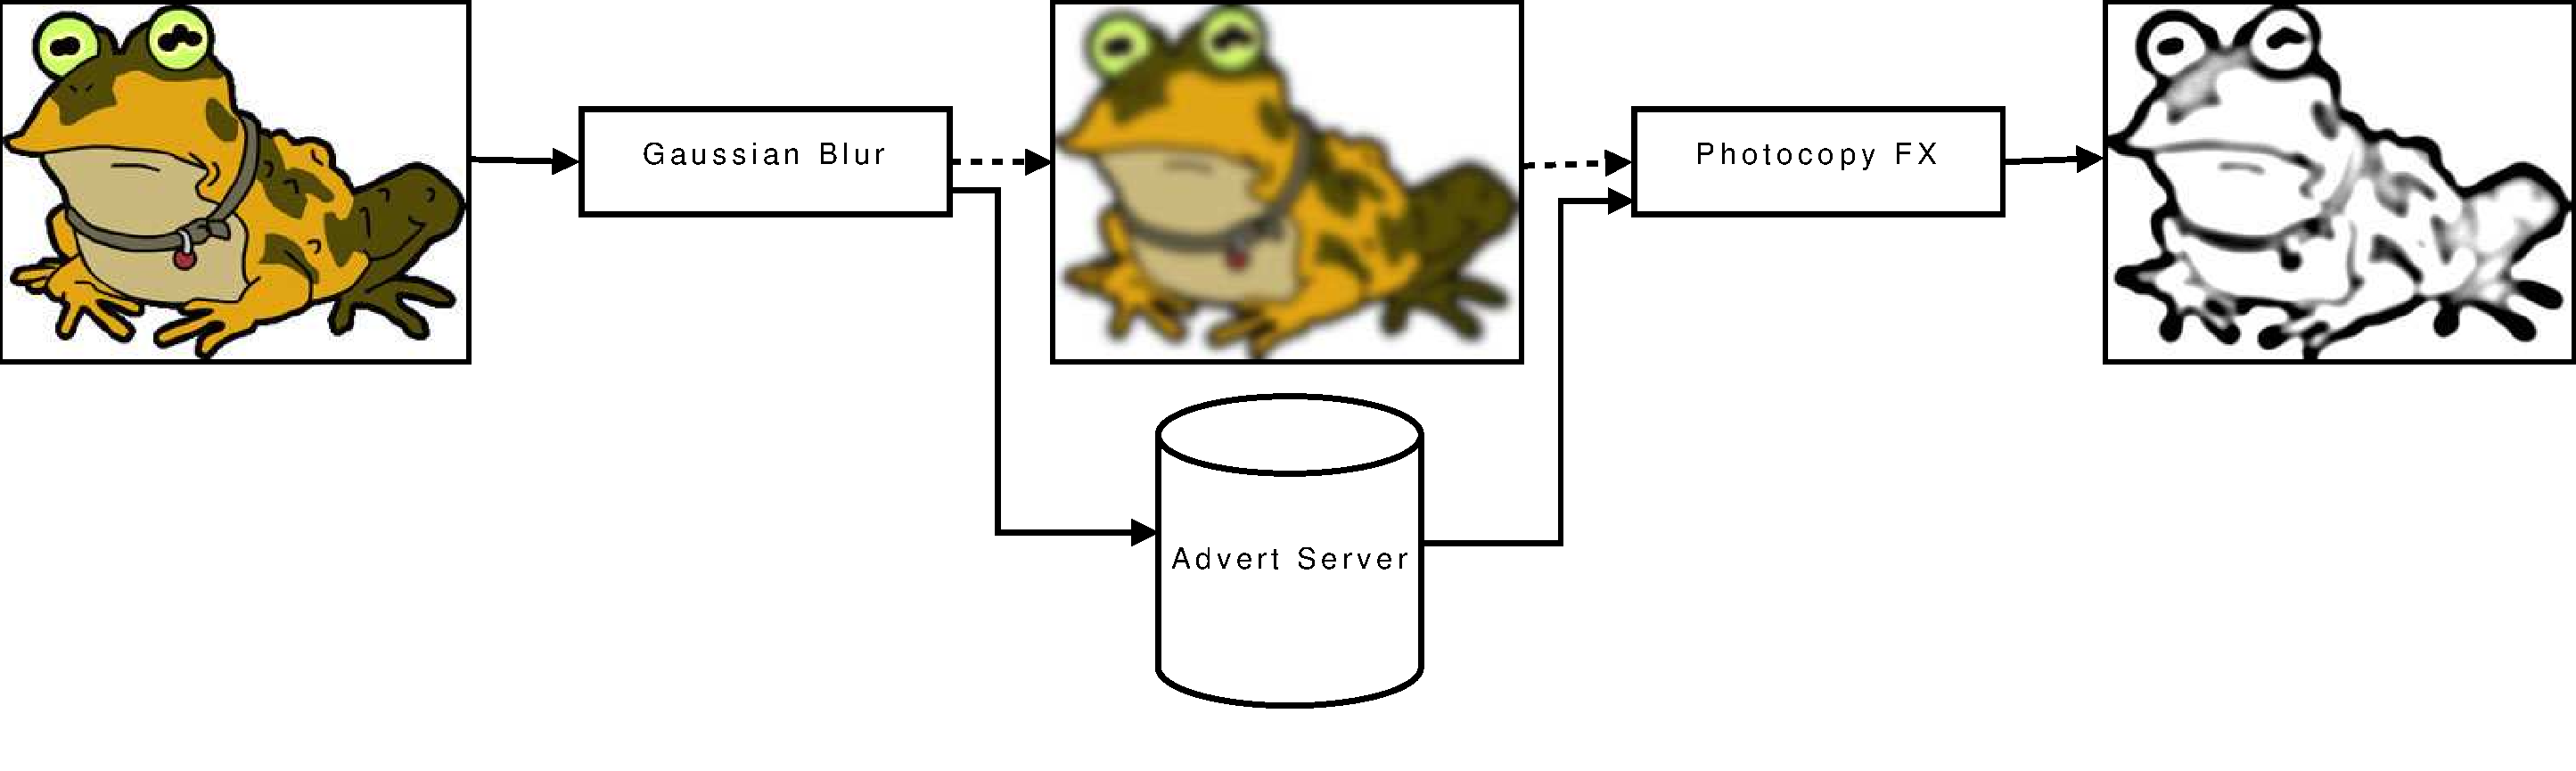
\includegraphics[width=14cm]{./figures/image_workflow.pdf} 
\caption{An Example of a Computational Workflow.\label{img-workflow}}
\end{center}
\end{figure*}

As an example for our application storage service, we took a closer look at
the \emph{JavaGAT AdvertService} \cite{javagat-www}. This provided us with main
functionality for our own Advert server, for adding, getting, deleting, and
finding objects in the Google datastore. Secondly we wrote a client library in
the Java programming language, which communicates over HTTP with the Advert
server, running at Google. Other Java programs can now use the client library
to store and retrieve (binary) application data at the Google App Engine.

As a result from building our Advert server similar to JavaGAT's AdvertService,
we could easily implement a JavaGAT AdvertService \emph{adaptor} for our
Google App Engine Advert server. Also we implemented a \emph{IPL server
bootstrap mechanism} for Ibis \cite{ipl-www}, where IPL servers can register
themselves in order to be found by other Ibis applications.

The rest of this paper is organized as follows. In Section \ref{related}
we look at related work, concerning \emph{Ibis} and the Google App Engine. In
Sections \ref{serverdesign} and \ref{serverimpl} we describe our Advert server
design and implementation, respectively, followed by the implementation of our
Advert client library in Section \ref{clientimpl}. Next we look at two
applications of Ibis in Section \ref{applications}. Finally we
present our benchmark results in Section \ref{benchmarks}, followed by our
conclusion and future work (Section \ref{conclusion}).
